% Denne fil er inkluderet i udtraekning_af_regioner.tex
{
Begrebet kantdetektion dækker over en metode som finder kanterne af
objekter i et billede. Egentlig prøver man at finde de punkter i
billedet, hvor kontrasten er stor, hvilket er tilfældet ved et objekts
grænse. Når vi har fundet kanterne til objekterne i billedet kan vi
bruge disse til at afgøre hvor vi har en ny region i billedet.  Som vi
skal se, så er kantdetektion et godt eksempel på hvor svært datamatsyn
kan være, selv i meget simple algoritmer.

\subsubsection*{Metode}
Der er forskellige algoritmer til rådighed for at finde kanter i
billeder\cite{SIOlsen}. Vi vil beskrive en meget naiv tilgang til
problemet, blot for at forklare grundprincipperne bag metoden. Som
allerede nævnt vil vi finde de steder i billedet hvor vi har stor
kontrast. Det er derfor almindeligt at konvertere billedet til sort/hvid
når man vil finde kanterne. Metoden forklares for én dimension, da det
let kan overføres til to dimensioner. Vi betragter derfor en vektor
$\mathbf{P}^t = (p_1, p_2, \cdots, p_n)$ som antager værdier i mængden
$\{0,1\}$.

\begin{figure}[!h]
    \renewcommand{\arraystretch}{1.5}
    \centering
    \begin{tabular}{|c|c|c|c|c|c|c|c|c|c|}
        \hline
        1 & 1 & 1 & 1 & 1 & \cellcolor{black}\textcolor{white}{0} & \cellcolor{black}\textcolor{white}{0} & \cellcolor{black}\textcolor{white}{0} & \cellcolor{black}\textcolor{white}{0} & 1\\\hline
    \end{tabular}
    \caption[]{Vektoren $\mathbf{P}^t$ med tilfældige værdier i mængden
    $\{0,1\}$.}
    \label{vektor_p_edge}
\end{figure}
Vektoren $\mathbf{P}$ kan betragtes som et liniestykke. Vi ønsker nu at
konstruere en ny vektor $\mathbf{E}^t = (e_1, e_2, \cdots, e_n)$, hvor
$e_i \in \{0,1\}$ ud fra vektoren $\mathbf{P}$. Vi definerer
$\mathbf{E}$ som
\begin{equation}
    \begin{split}
        \mathbf{E}^t &= (e_1, e_2, \cdots, e_n) \mathrm{~,~hvor~} \\
        &e_i = \left\{
        \begin{array}{rl}
            0 & \text{hvis~} |p_i - p_{i - 1}| = 1\\
            1 & \text{hvis~} |p_i - p_{i - 1}| = 0
        \end{array} \right. \mathrm{,~for~} p_i \subseteq \mathbf{P}
        \mathrm{~og~} p_0 = p_1
    \end{split}
    \label{vektor_e_bin}
\end{equation}
Vektoren $\mathbf{E}$ konstrueres altså ved at sammenligne et givet
punkts værdi med det forrige punkts værdi. Hvis den absolutte forskel
til et punkts forgænger er lig $1$ så sættes dette punkt til værdien $0$
i kantvektoren $\mathbf{E}$. Hvis der ikke er nogen forskel sættes værdien til
$1$. Vi er i denne sammenhæng nødt til at definere $p_0$ til $p_1$, så
vi undgår at finde en kant i starten af en linie. Kantvektoren
$\mathbf{E}$ for $\mathbf{P}$ er vist i figur \ref{vektor_e_edge}.

\begin{figure}[!h]
    \renewcommand{\arraystretch}{1.5}
    \centering
    \begin{tabular}{|c|c|c|c|c|c|c|c|c|c|}
        \hline
        1 & 1 & 1 & 1 & 1 & \cellcolor{black}\textcolor{white}{0} & 1 &
        1 & 1 & \cellcolor{black}\textcolor{white}{0} \\\hline
    \end{tabular}
    \caption[]{Kantvektoren $\mathbf{E}$ for $\mathbf{P}$.}
    \label{vektor_e_edge}
\end{figure}
Det ses at $e_6 = e_{10} = 0$, da $|p_6 - p_5| = |p_{10} - p_9| = 1$. Vi
har nu markeret de steder hvor der er kontrast i den oprindelige vektor
$\mathbf{P}$. Vi gør os en vigtig observation vedrørende definitionen på
$\mathbf{E}$. Vi markerer en kant i det punkt hvor kontrasten netop
\emph{er} skiftet. Derfor har vi også at $e_{10}$ bliver markeret som en
kant, selvom man ved manuel inspektion ville markere $e_9$ som kanten.
Dette skyldes at vi ikke har nogen hukommelse i definitionen og derfor
ikke er klar over hvilke punkter der burde hænge sammen. Vi ved altså
ikke hvilke værdier der er de interessante. Denne problematik
understreges af det faktum, at end ikke mennesket altid kan afgøre hvor
grænsen mellem to figurer går. Et klassisk eksempel er den optiske
illusion ved \emph{Rubins vase}\cite{WikiRubinVase} vist i figur
\ref{rubins_vase}. Alt efter hvad man vælger som fokus i billedet, vil
kanten skulle redefineres.

\begin{figure}[!h]
    \begin{center}
        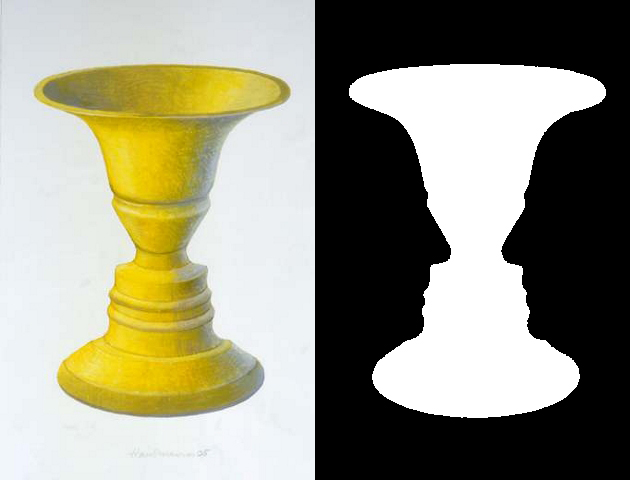
\includegraphics[trim = 84mm 4mm 0mm 0mm, clip, width=3cm]{afsnit/vores_implementation/billeder/kantdetektion/Rubin2}
    \end{center}
    \caption[]{Rubins vase\cite{WikiRubinVasePic}.}
    \label{rubins_vase}
\end{figure}

Vi kan generalisere definitionen for kantvektoren $\mathbf{E}$ i
\ref{vektor_e_bin} således at vi kan have andre værdier end dem i
$\{0,1\}$ og en anden tærskelværdi. I den følgende definition har vi at
$t$ angiver den tærskelværdi, for hvor meget værdierne punkterne imellem
må afvige.
\begin{equation}
    \begin{split}
        \mathbf{E}^t &= (e_1, e_2, \cdots, e_n) \mathrm{~,~hvor~} \\
        &e_i = \left\{
        \begin{array}{rl}
            0 & \text{hvis~} |p_i - p_{i - 1}| \geq t\\
            1 & \text{hvis~} |p_i - p_{i - 1}| < t
        \end{array} \right. \mathrm{,~for~} p_i \subseteq \mathbf{P}
        \mathrm{~og~} p_0 = p_1
    \end{split}
    \label{vektor_e_generel}
\end{equation}

Definitionen på $\mathbf{E}$ tager ikke højde for støj i billedet,
hvilket let kan forvirre kantdetektionen. Sobels algoritme er en
etableret metode til at finde kanter i billeder som benytter to
foldningsmatricer til at finde kanter vertikalt og horisontalt. Den
lider dog under samme svaghed for støj som den simple metode[ref]. Vi
vil benytte os af en metode udviklet af John F. Canny som kombinerer
metoder fra bla. gaussisk sløring og Sobel[ref]. Vi vil ikke komme
nærmere ind på den indre funktionalitet i Canny, men vi vil i det
følgende vise eksempler på resultater fra metoden.

\subsubsection*{Eksempler}

\begin{figure}[!h]
    \begin{center}
        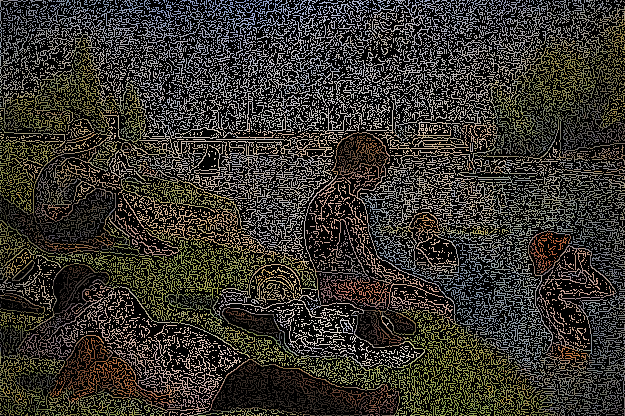
\includegraphics[width=0.8\textwidth]{afsnit/vores_implementation/billeder/kantdetektion/canny_20_20}
    \end{center}
    \caption[]{Canny kantdetektion med tærskelværdierne $(20, 20)$.}
    \label{bathers}
\end{figure}
}

% vim: set tw=72 spell spelllang=da:
